
\section{Evaluaci�n de estrategias}

\subsection{File Scan}

La traza del \fs no tendr� HITs para ning�n tipo de algoritmo de reemplazo de p�ginas porque \fs pide UNA sola vez cada p�gina.\\
Por otro lado, se observaron resultados interesantes cuando hac�amos traces que le�an 2 veces el mismo archivo y comparab�mos los hit-rates de las diferentes estatregias, de estos resultados obtuvimos las siguientes conclusiones:

\begin{itemize}
\item LRU y FIFO tienen el mismo comportamiento durante un \fs porque l�s p�ginas que se eligen para desalojar en ambos casos son las primeras en haber sido referidas.
\item Si hab�a igual o m�s cantidad de frames, el hit-rate pasaba a ser del 50\% para todas las estrategias, porque si bien en la primera pasada todas las referencias a p�ginas era misses, para la segunda estaban todos en memoria.
\item Para una cantidad de p�ginas superior en una unidad a la cantidad de frames, LRU ten�a 100\% de miss-rate(y por ende tambi�n la estrategia FIFO). Esto se debe a que necesita desalojar el primer frame para alojar la �ltima p�gina(en la primera pasada); luego, cuando necesitaba leer nuevamente la primera p�gina(en la segunda pasada) tiene que desalojar el �ltimo frame en ser accedido(el segundo), para el segundo el tercero, y as� sucesivamente.
\item Las estrategias empiezan a convergen en torno a un hit-rate del 50\% cuando la cantidad de frames se acerca a la cantidad de p�ginas dado que es necesario desalojar menos frames.
\item Entre las estrategias evaluadas, la �nica que mejora el hit-rate cuando la cantidad de frames es menor a la cantidad de p�ginas a ser le�das es MRU. 
\end{itemize}

\begin{center}
\huge File Scan\\
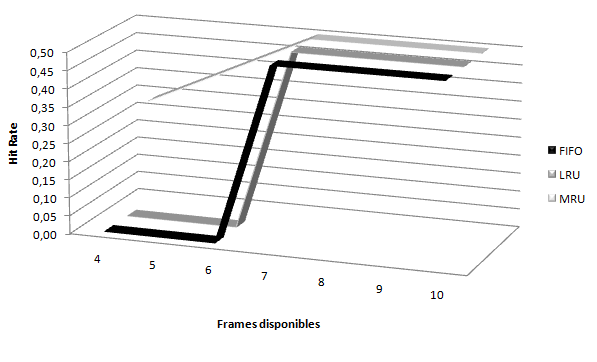
\includegraphics[scale=0.75]{img/fileScan2Times.png}
\end{center}

\subsection{Index Scan Clustered}

El ejemplo dado por la catedra no reutiliza ninguna pagina, por lo que estudiar 

